% !TeX root = ../main.tex
% 修改稿迁移版：自动编号，原文数据与待核事项保留。
\chapter*{证明材料}
\addcontentsline{toc}{chapter}{证明材料}
\renewcommand{\theHfigure}{appendix.\arabic{figure}}
\renewcommand{\theHtable}{appendix.\arabic{table}}
\begin{figure}[H]\centering
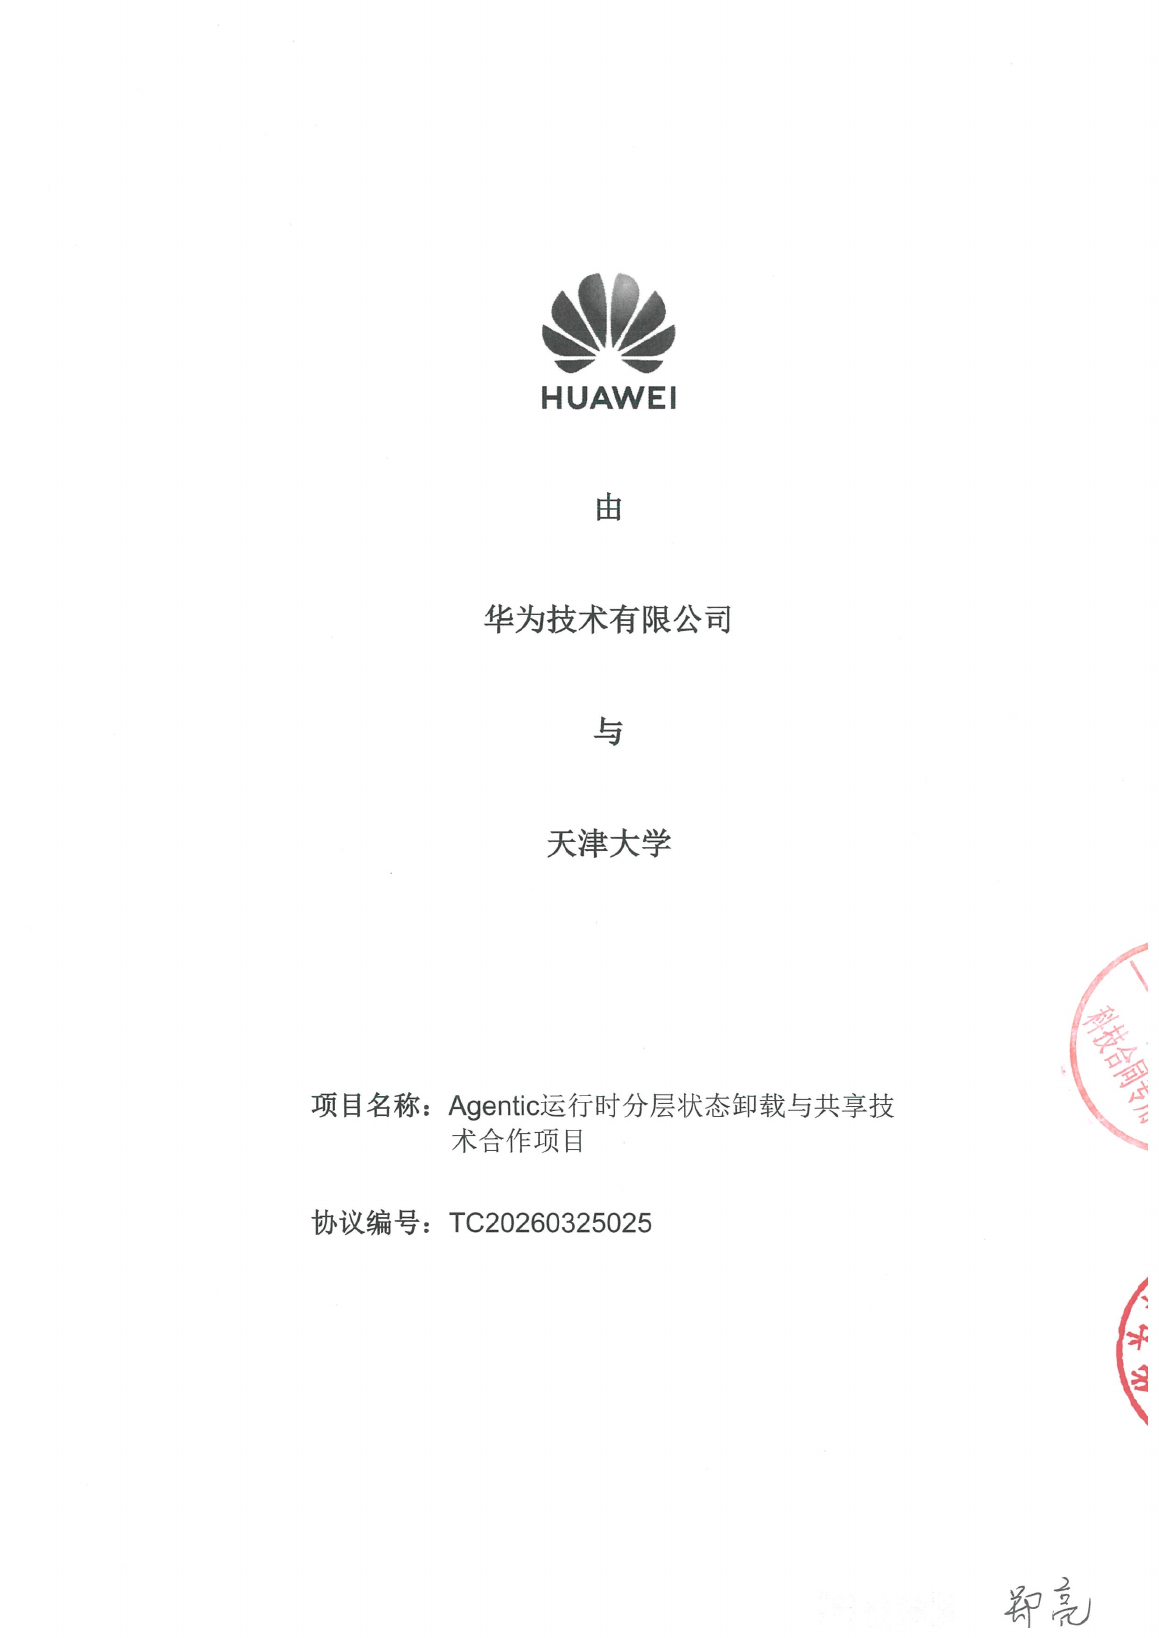
\includegraphics[width=\linewidth,height=.83\textheight,keepaspectratio]{figures/image27.png}
\caption*{证明材料 1 技术合作项目协议封面}
\end{figure}\clearpage
\begin{figure}[H]\centering
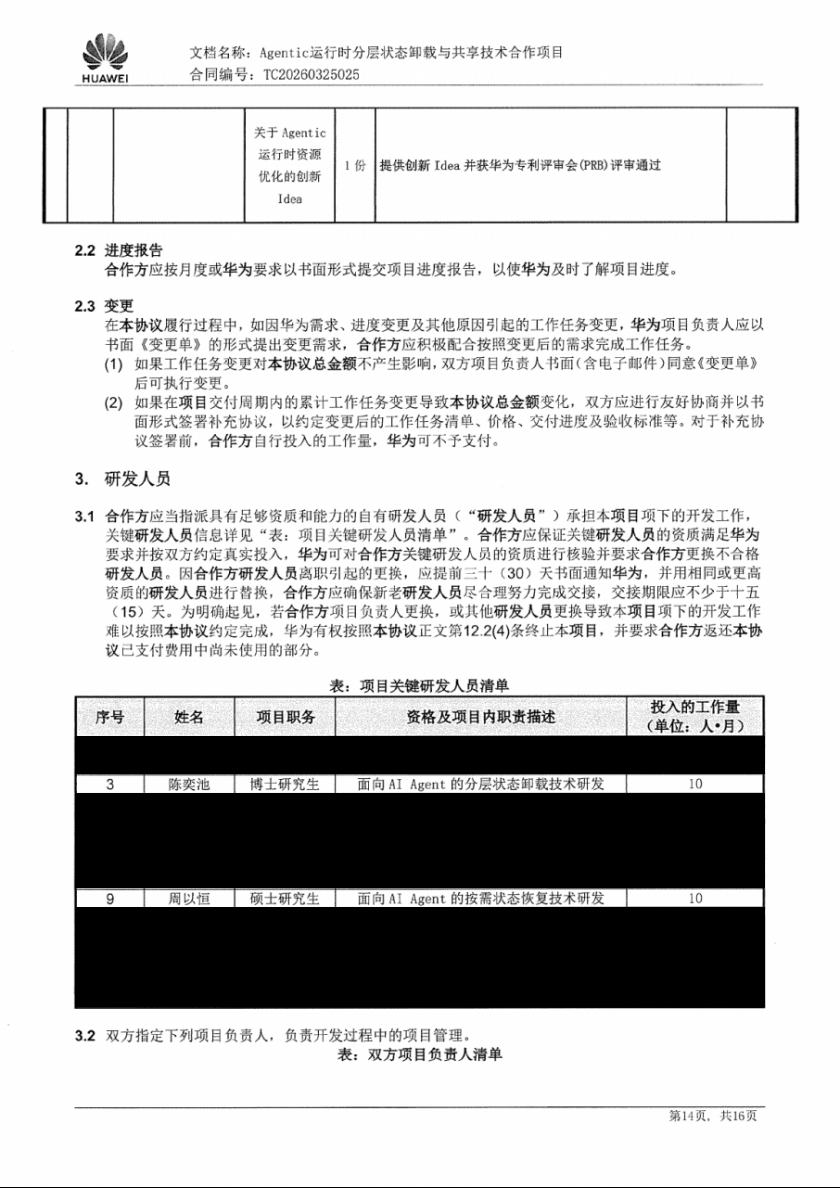
\includegraphics[width=\linewidth,height=.83\textheight,keepaspectratio]{figures/image28.png}
\caption*{证明材料 2 项目关键研发人员}
\end{figure}\clearpage
\section*{证明材料边界说明}
\addcontentsline{toc}{section}{证明材料边界说明}
为避免证明材料被过度解读，本节按“材料---性质---可支撑的结论---不能支撑的结论”说明各项材料的使用边界。三项边界原则是：区分直接项目证据与相关技术积累；区分合同阶段成果与产品最终验收成果；区分研究环境测试结果与华为指定环境下的结果。对外材料与答辩表述均以本节口径为准。

\FloatBarrier
\begingroup\linespread{1}\selectfont
\renewcommand{\thetable}{A-\arabic{table}}\setcounter{table}{0}
\begin{longtable}{@{}>{\raggedright\arraybackslash}p{\dimexpr 0.19531\linewidth-1.1719\tabcolsep\relax}>{\raggedright\arraybackslash}p{\dimexpr 0.15191\linewidth-0.9115\tabcolsep\relax}>{\raggedright\arraybackslash}p{\dimexpr 0.30382\linewidth-1.8229\tabcolsep\relax}>{\raggedright\arraybackslash}p{\dimexpr 0.34896\linewidth-2.0938\tabcolsep\relax}@{}}
\caption{证明材料边界与可支撑结论}\label{tab:A-1}\\
\hline
\rowcolor{WordTableHeader} \TableHeaderText{材料} & \TableHeaderText{材料性质} & \TableHeaderText{可支撑的结论} & \TableHeaderText{不能支撑的结论} \\ \hline
\endfirsthead
\multicolumn{4}{c}{\fontsize{9}{12}\selectfont 表 A-1（续）}\\
\hline
\rowcolor{WordTableHeader} \TableHeaderText{材料} & \TableHeaderText{材料性质} & \TableHeaderText{可支撑的结论} & \TableHeaderText{不能支撑的结论} \\ \hline
\endhead
\hline\endfoot\hline\endlastfoot
\rowcolor{WordTableStripe} 
天津大学与华为技术合作项目协议及关键研发人员页 & 直接项目证据 & 项目依托天津大学与华为签署的校企科研合作项目开展；协议约定研发经费 113.3 万元（含税）；列明了承担研究任务的核心研发人员 & 不能说明学生团队直接与华为签订合作合同；该经费不计入创业企业销售收入，也不等同于已到账资金 \\ \hline
项目阶段报告与测试记录 & 项目进展证据 & 已完成核心代码开发与系统设计材料，并完成研究环境下的阶段测试；48 个任务并发测试全部完成且未发生内存不足导致的中断 & 不能作为华为指定环境下的验收结论；相关指标以研究环境为测试条件，指标口径见各表说明 \\ \hline
\rowcolor{WordTableStripe} 
华为 FunctionGraph 应用证明 & 历史技术积累证据 & 团队在相关技术方向具备产业应用经历 & 不是 PI OS 的应用证明，不能说明 PI OS 已在华为平台落地 \\ \hline
腾讯 UNMOOR 应用证明 & 相关技术产业验证证据 & 内存管理相关技术方向已获得产业验证 & 不是 PI OS 的客户或收入证明，不能说明 PI OS 已在腾讯落地或已产生收入 \\ \hline
\rowcolor{WordTableStripe} 
代码与文档版本记录、实验脚本与复现说明 & 过程性证据 & 学生承担了具体的实现、实验与复核工作，实验结果为项目组自行复核，可由他人按说明复现 & 不能替代第三方验收或客户使用证明，不等同于外部机构的检测结论 \\ \hline
\end{longtable}\endgroup
项目在后续提交与答辩中，将按上述边界使用全部材料。如取得新的验收结论、客户试点数据或授权文件，将及时更新本节内容与表 1-1 的证据索引。

图 A-1 以分层方式呈现不同性质材料的证据强度差异。

\begin{figure}[H]\centering
\renewcommand{\thefigure}{A-\arabic{figure}}\setcounter{figure}{0}
\begin{tikzpicture}[x=1cm,y=1cm,every node/.style={font=\fontsize{9}{11}\selectfont\linespread{1}\selectfont,align=center},box/.style={draw=DiagramRule,rounded corners=2pt,fill=DiagramLight,inner sep=4pt},arr/.style={->,>=stealth,draw=DiagramMain}]
\node[box,text width=5.8cm,dashed,fill=white] (l0) at (3.2,0) {\textbf{1 外部验收与客户证据}\\待形成；现有合同与内部测试不能替代};
\node[box,text width=5.8cm,fill=DiagramMain,text=white] (l1) at (9.8,0) {\textbf{2 合同与授权证据}\\合作协议已形成；商用授权仍需核查};
\node[box,text width=5.8cm,fill=DiagramMedium] (l2) at (9.8,-1.65) {\textbf{3 项目进展证据}\\阶段报告与内部测试；不等于最终验收};
\node[box,text width=5.8cm] (l3) at (3.2,-1.65) {\textbf{4 过程性证据}\\代码、复现脚本与培训会议记录};
\draw[arr] (l0) -- (l1);\draw[arr] (l1) -- (l2);\draw[arr] (l2) -- (l3);
\node[box,text width=12.4cm] (note) at (6.5,-3.1) {历史产业应用证明用于说明相关技术积累，置于直接项目证据之外；各类材料可支撑结论见表 A-1。};
\end{tikzpicture}
\caption{证明材料证据强度分层图}\label{fig:A-1}
\end{figure}

\clearpage
\section*{补充证明材料}
\addcontentsline{toc}{section}{补充证明材料}
本节保留模板原有的相关技术产业应用证明。它们用于说明相关技术积累，不作为 PI OS 的客户、销售收入或平台落地证明，使用边界见表 A-1。
\begin{figure}[H]\centering
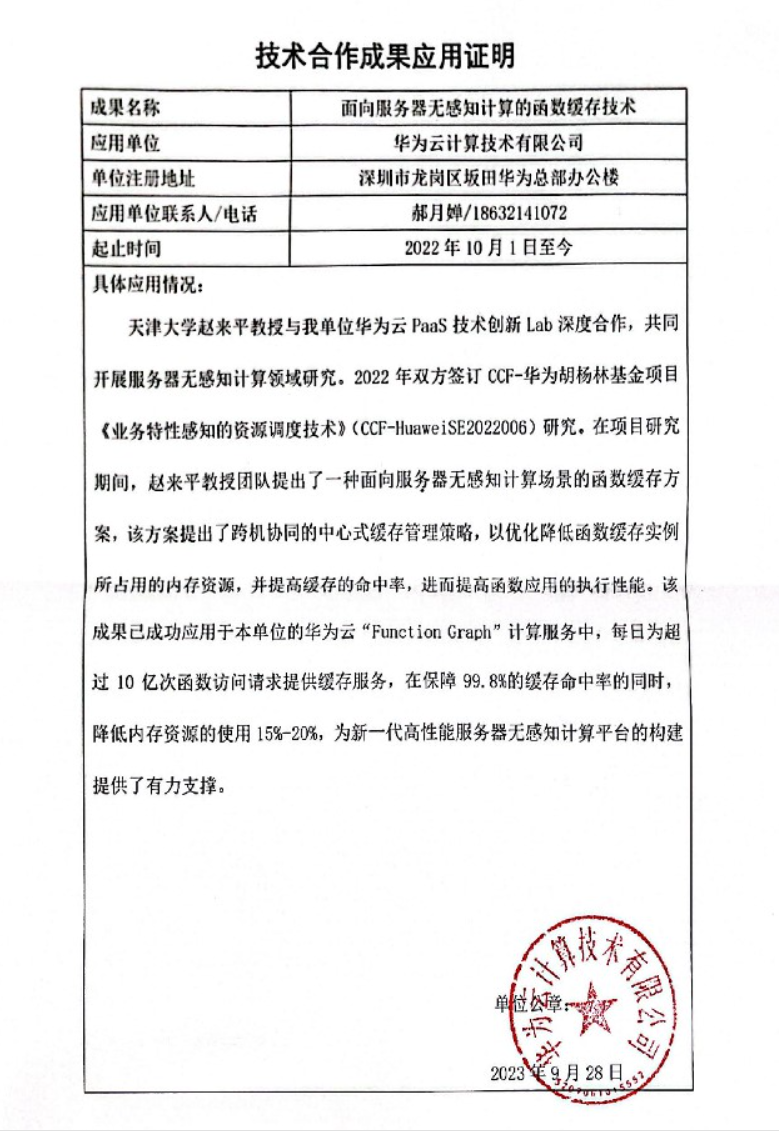
\includegraphics[width=\linewidth,height=.83\textheight,keepaspectratio]{figures/evidence-huawei.png}
\caption*{证明材料 3 华为 FunctionGraph 相关技术应用证明}
\end{figure}\clearpage
\begin{figure}[H]\centering

\includegraphics[width=\linewidth,height=.83\textheight,keepaspectratio]{figures/evidence-tencent.pdf}
\caption*{证明材料 4 腾讯 UNMOOR 相关技术应用证明}
\end{figure}
